\subsection{Die Strahlungsprozesse der Erde}

\begin{frame}
	\frametitle{Aufbau der Atmosphäre}
	\begin{figure}
		\centering
    \begin{columns}
      \column{0.1\linewidth}
      \column{0.5\linewidth}
      \begin{tikzpicture}
		    \node[anchor=south west,inner sep=0] (image) at (0,0) {
        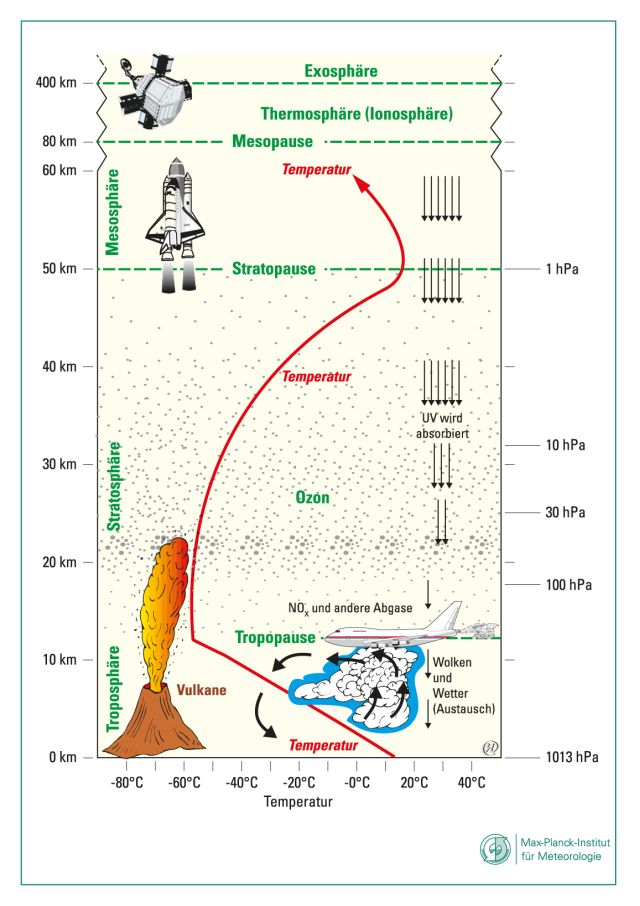
\includegraphics[width=.85\linewidth]{bilder/atmosphaere-stockwerkaufbau_bildungsserver_hh.jpg}};
        \begin{scope}[x={(image.south east)},y={(image.north west)}]
        \onslide<2|handout:0>\draw[red,ultra thick,rounded corners] (0.05,0.15) rectangle (0.95,0.285);
        \onslide<3|handout:0>\draw[red,ultra thick,rounded corners] (0.05,0.285) rectangle (0.95,0.715);
        \onslide<4|handout:0>\draw[red,ultra thick,rounded corners] (0.05,0.715) rectangle (0.95,0.855);
        \onslide<5|handout:0>\draw[red,ultra thick,rounded corners] (0.05,0.855) rectangle (0.95,0.96);
    \end{scope}
      \end{tikzpicture}
      \column{0.3\linewidth}
        \caption{Schematischer Aufbau der Atmosphäre, Quelle: Bildungsserver Hamburg}
      \column{0.1\linewidth}
    \end{columns}
	\end{figure}

  \note<2>{
    Troposphäre, \SIrange{10}{12}{km}
    \begin{itemize}
      \item[] \SI{80}{\%} der Atmosphärenmasse, enthält fast allen Wasserdampf
      \item[] Hier finden alle wetterrelevanten Phänomene statt
      \item[] ersten \SIrange{1}{2,5}{km} starker Einfluss der Erdoberfläche
      \item[] Jetstreams an oberer Grenze, kein Transport von H$_2$0 von Troposphäre in die Stratosphäre
    \end{itemize}
		}
	\note<3>{
    Stratosphäre, \SIrange{12}{50}{km}
    \begin{itemize}
      \item[] Anstieg der Ozonkonzentration sorgt für Temperaturanstieg
      \item[] Die Prozesse hier (Strahlung, Dynamik, Chemie) relevant für Klima in der Troposphäre
    \end{itemize}
		}
	\note<4>{
    Mesosphäre, \SIrange{50}{80}{km}
    \begin{itemize}
      \item[] Stetige Temperaturabnahme
    \end{itemize}
		}
	\note<5>{
    Thermosphäre, \SIrange{80}{400}{km}
    \begin{itemize}
      \item[] extrem geringe Teilchendichte, Weltram fängt bei \SI{100}{km} an (NASA), Bremswirkung der Atmosphäre aber auch bei \SI{400}{km} Höhe noch spührbar (ISS wird regelmäßig von andockenden Raumschiffen auf ihre Bahn zurück geschoben)
    \end{itemize}
    Exosphäre, \SIrange{400}{1000}{km}
    \begin{itemize}
      \item[] quasi Vakuum
    \end{itemize}
    Grenzen nicht hart, Troposphäre z.B.
    \begin{itemize}
      \item[] 10-12 km im Durchschnitt
      \item[] 8 km an den Polen
      \item[] 17-18 km in den Tropen
    \end{itemize}
  }
\end{frame}

%Übergang: Ohne die Atmosphäre hätten wir auf der Erde eine durchschnittliche Temperatur von -18 Grad, durch die Atmosphäre und die atmosphärischen Gase ist es aber im Mittel etwa etwa 35 Grad wärmer -> 15 Grad

\begin{frame}
  \frametitle{Strahlungshaushalt}

  \begin{figure}
  	\centering
    \begin{tikzpicture}
      \node[anchor=south west,inner sep=0] (image) at (0,0){
  	   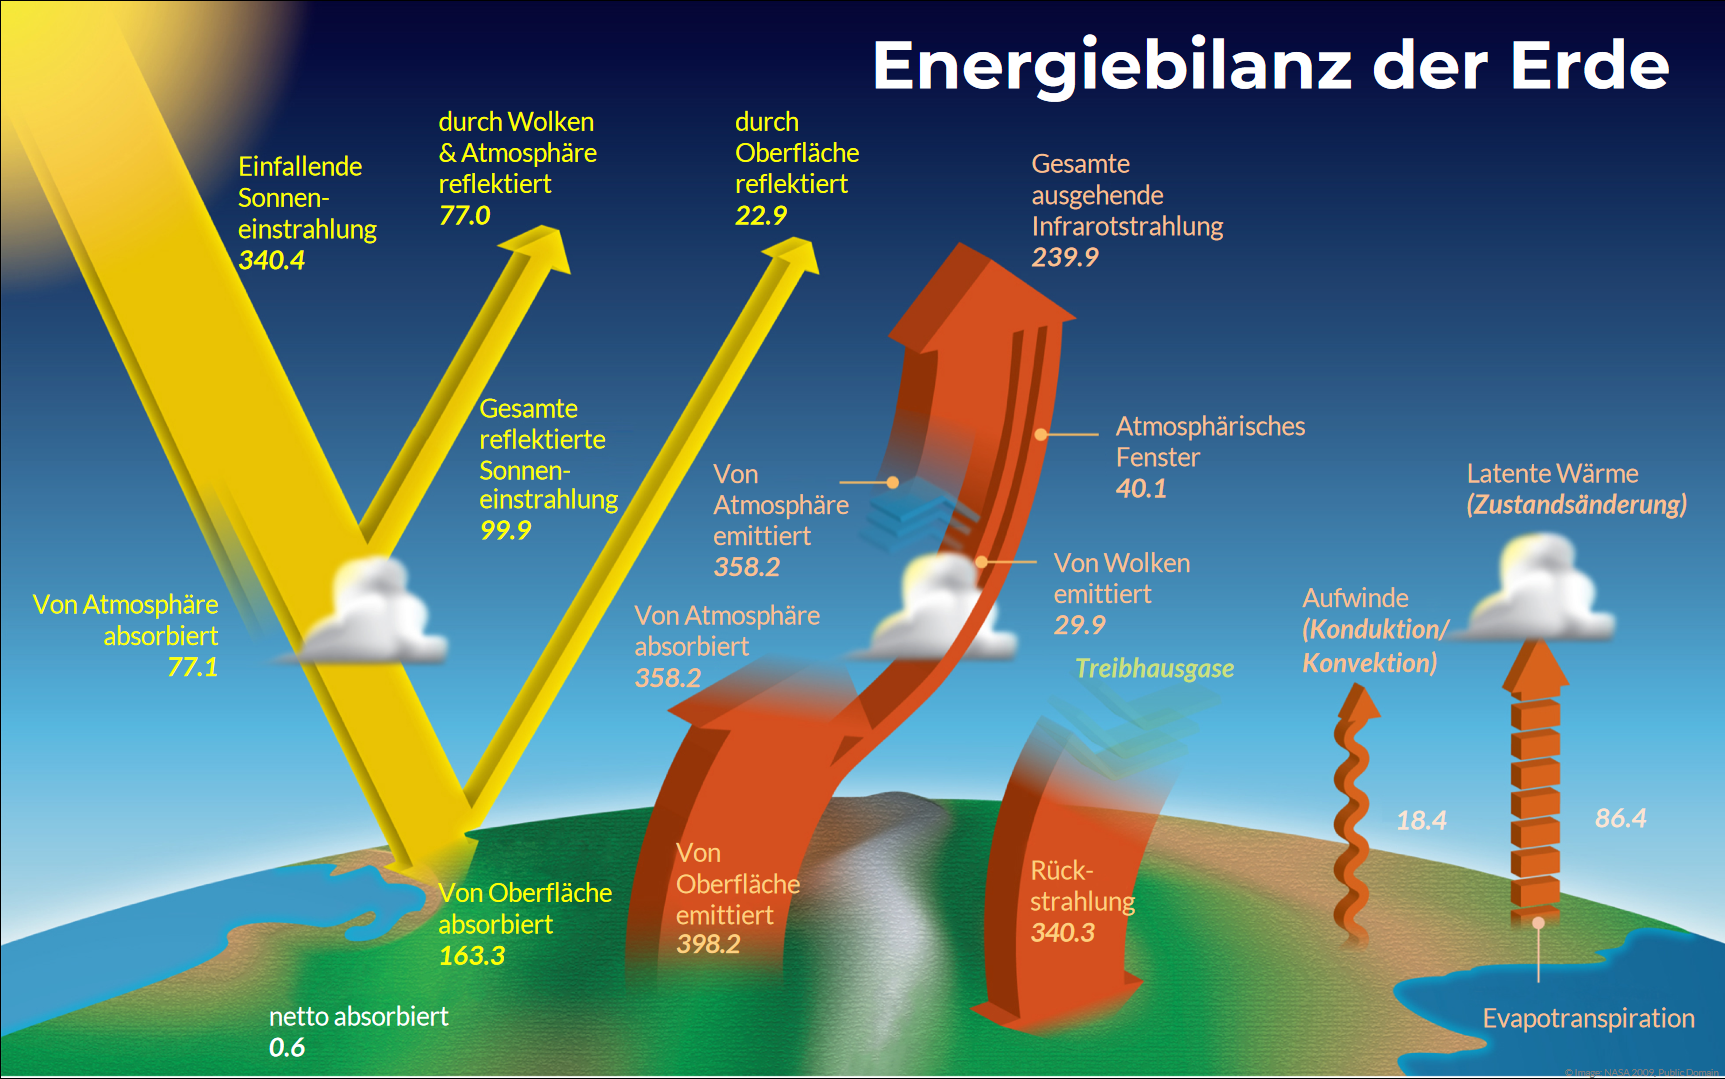
\includegraphics[width=0.8\linewidth]{bilder/Energiebilanz_der_Erde_NASA.png}};
      \uncover<2->{
        \node[anchor=south west, text=red] (text) at (4.7, 3.235) {\scriptsize\textbf{\rule[0.5ex]{2em}{0.55pt}\;\num{169.9}}};
      }
    \end{tikzpicture}
  	\caption{Strahlungshaushalt der Erde, Angaben in W/m$^2$, Quelle: NASA nach Kiehl und Trenberth 1997, Übersetzung: S4F} % Die Abbildung ist in den Folien der S4F Vertiefung zum Klimawandel (S.21) aber dort leider nur spärlich referenziert. Annahme: Jemand der S4F hat dieses Bild Übersetzt und dem Abbildungs-Pool hinzugefügt.
  \end{figure}

  %Abbildung für Strahlungshaushalt einfügen z.B: vom Bildungsserver Hamburg https://bildungsserver.hamburg.de/atmosphaere-und-treibhauseffekt/2069644/atmosphaere-strahlungshaushalt-artikel/
  % bzw. vom den S4F materialien: http://files.scientists4future.org/Themen/2.%20Klimawandel/Als%20PDFs/S4F-03%20Klima%20Vertiefung%202020-01-31.pdf
  % oder vom IPCC AR5 Figure 2.11
  \note<1->{
  \begin{itemize}
    \item[] Ohne die Atmosphäre hätten wir eine durchschnittliche Oberflächentemperatur von \SI{-18}{°C}
    \item[] Mit Atmosphäre (Treibhausgase) ist es im Mittel \SI{33}{°C} wärmer, wir haben eine durchschnittliche Oberflächentemperatur von \SI{15}{°C}
    \item[] Solarkonstante: \SI{1368}{W\per m\squared} oberhalb der Atmosphäre
    \begin{itemize}
      \item[] Zur Erwärmung der Atmosphäre verfügbar: \SI{340}{W\per m\squared} auf Grund der Kugelgestalt und der Nachtseite der Erde
      \item[] rund \SI{70}{\%} der gesamten einfallenden Strahlung werden absorbiert (Atmosphäre (\SI{22}{\%}), Oberfläche (\SI{48}{\%}))
      \item[] rund \SI{30}{\%} der gesamten einfallenden Strahlung werden reflektiert (Wolken und Atmosphäre (\SI{23}{\%}), Erdoberfläche (\SI{7}{\%}))
    \end{itemize}
	\end{itemize}
	}
	\note<2->{
	\begin{itemize}
    \item[] Damit sich die Erde nicht aufheizt, muss die absorbierte Energie wieder abgegeben werden
    \item[$\rightarrow$] Die absorbierte kurzwellige Sonneneinstrahlung wird als langwellige infrarot Strahlung wieder abgegeben (vgl. Eingehend \SI{340}{W\per m\squared} und Ausgehend \SI{100}{W\per m\squared} reflektiert, sowie \SI{240}{W\per m\squared} als IR abgestrahlt)
    \item[] Zusätzlich \SI{340}{W\per m\squared} Rückstrahlung $\rightarrow$ Woher kommen die?
    \begin{itemize}
      \item[] Einergiebilanz der Atmosphäre: \SI{77}{W\per m\squared} Sonneneinstrahlung + \SI{358}{W\per m\squared} Erdeinstrahlung + \SI{18}{W\per m\squared} Aufwinde + \SI{86}{W\per m\squared} latente Wärme - \SI{200}{W\per m\squared} von Wolken und Atmosphäre emittiert = \SI{340}{W\per m\squared} bleiben übrig
      \item[$\rightarrow$] Treibhauseffekt
			\item[$\rightarrow$] zuvor: Exkurs Licht
    \end{itemize}
  \end{itemize}
  }
\end{frame}
